\documentclass[10pt,ps,serif,mathserif]{beamer}
\usepackage[utf8]{inputenc} % указывает кодировку документа
\usepackage[T2A]{fontenc} % указывает внутреннюю кодировку TeX 
\usepackage[russian]{babel} % указывает язык документа
\usetheme{Warsaw}
\usepackage{graphicx}
\usepackage{multirow}
\usepackage{enumerate}
\usepackage{enumitem}
\usepackage{listings}
\usepackage{longtable}
\usepackage{mathtools}
\usepackage{verbatim}
\usepackage{color, colortbl}

\begin{document}
\def\labelenumi{\theenumi}
\def\labelenumii{\theenumii}
\def\labelitemi{\theenumi}
\renewcommand{\theenumi}{\arabic{enumi}}
\renewcommand{\labelenumi}{\theenumi)}
\renewcommand{\theenumii}{\alph{enumii}}
\renewcommand{\labelenumii}{\arabic{enumi}.\arabic{enumii}}
\renewcommand{\labelitemi}{$\bullet$}


\title[Определение перечислений на английском языке]{Определение перечислений в предложениях на английском языке на основе их синтаксического анализа}
\author[Клевцов В.А.]{Исполнитель: Клевцов В.А.}
\date{}
\institute{\normalsize Волгоградский государственный технический университет \\
        \vspace{0.7cm}
            Научный руководитель:  к.т.н. Сычев О.А.\\
                \vspace{0.7cm}
            }
\setbeamertemplate{navigation symbols}{%
    \setbeamercolor{footline}{fg=black}
    \setbeamerfont{footline}{series=\bfseries}
    \usebeamerfont{footline}%
    \usebeamercolor[fg]{footline}%
    \hspace{1em}%
}
    \begin{frame}
        \titlepage
    \end{frame}
\setbeamertemplate{navigation symbols}{%
    \setbeamercolor{footline}{fg=black}
    \setbeamerfont{footline}{series=\bfseries}
    \usebeamerfont{footline}%
    \usebeamercolor[fg]{footline}%
    \hspace{1em}%
    \normalsize \insertframenumber/\inserttotalframenumber
}
    \begin{frame}{Актуальность}
        \begin{block}{Вопрос}
        Составьте предложение из слов: <<Vasya>> , <<went>> , <<park>> , <<John>> , <<and>> , <<to>> , <<the>>, <<and>> , <<cinema>> , <<to>> , <<the>>.
        \end{block}
        \begin{block}{Ответ}
        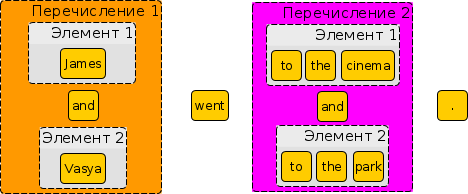
\includegraphics[width=\textwidth]{images/answer.png}
        \end{block}
    \end{frame}
    \begin{frame}{Постановка проблемы}
        \begin{block}{Проблема}
            Трудоемкость создания вопросов, ответами на которые являются предложения с однородными членами и/или сложносочиненными предложениями.
        \end{block}

        \begin{block}{Подходы к решению}
            \begin{enumerate}
                \item Отказ от использования вопросов с ответами содержащими однородные члены и/или сложносочиненные предложения.
                \item Вручную вводить каждый вариант правильного ответа.
                \item {\color{magenta} Использовать автоматизированное определение перечислений}
            \end{enumerate}
        \end{block}
    \end{frame}
    \begin{frame}{Постановка задачи}
        \small
        \textbf{Дано:} T = <A,S,E,t> \\
        
        \hspace{0.5cm}\textbf{T} - Эталонный ответ \\
        \hspace{0.5cm}\textbf{A} - Множество лексем эталонного ответа\\
        \hspace{0.5cm}\textbf{S} - Множество описаний лексем эталонного ответа \\
        \hspace{0.5cm}\textbf{E} - Множество описаний перечислений содержащихся в правильном ответе \\
        \hspace{0.5cm}\textbf{t} - Трудоемкость создания эталонного ответа на вопрос \\
        \(t = t_{A} + t_{S} + t_{E}\) \\
        \hspace{0.5cm}\(\mathbf{t_A}\) - Трудоемкость ввода лексем эталонного ответа\\
        \hspace{0.5cm}\(\mathbf{t_S}\) - Трудоемкость ввода описаний лексем эталонного ответа \\
        \hspace{0.5cm}\(\mathbf{t_E}\) - Трудоемкость ввода описаний перечислений содержащихся в правильном ответе \\
        \textbf{Цель:} минимизировать t. \\
        \textbf{Решение:} 
        Разработать функцию: F(A) \\
        \hspace{0.5cm}\textbf{F} - Функция генерации множества описаний перечислений содержащихся в правильном ответе.\\
        Новая трудоемкость будет определяться формулой:\\
        \(t = t_{A} + t_{S} + t_{eE},  ~ \forall{A}, ~t_{E} \ge t_{eE} \) \\
        \hspace{0.5cm}\(\mathbf{t_{eE}}\) - Трудоемкость редактирования автоматически определенных описаний перечислений содержащихся в правильном ответе \\
        
    \end{frame}
    \begin{frame}{Описание предметной области}
        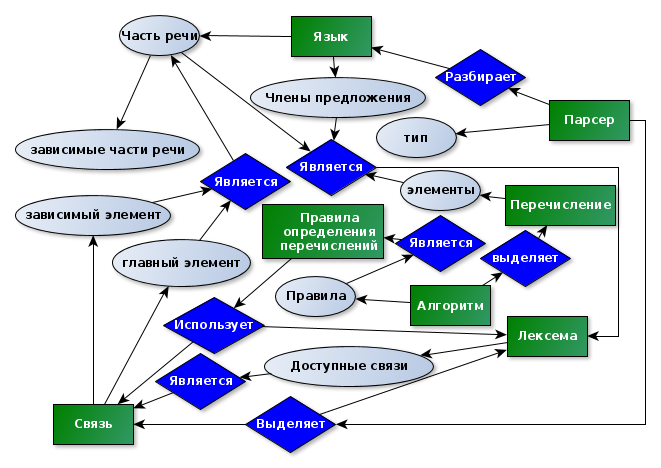
\includegraphics[width=\textwidth]{images/erd.png}
    \end{frame}
    \begin{frame}{Цель}
        \Large Целью работы является снижение трудоемкости создания вопросов типа Correct Writing для
        СУО Moodle за счет автоматического определения перечислений в английском языке на основе синтаксического
        анализа предложения.
    \end{frame}
    \begin{frame}{Задачи}
        \large
       \begin{enumerate}
        \item исследовать подходы, методы и средства обработки естественных языков,
                выбрать программное средство для осуществления синтаксического анализа;
        \item исследовать правила английского языка, выбрать структуры языка, изменение порядка записи
            которых, не изменяют семантику предложения;
        \item разработать метод выделения перечислений в английском языке на основе синтаксического
            анализа;
        \item реализовать и интегрировать метод в плагин Correct Writing, провести тестирование и
            эксперимент, оценить достижение цели.
       \end{enumerate}
    \end{frame}
    \begin{frame}{Обзор существующих методов анализа естественного языка}
        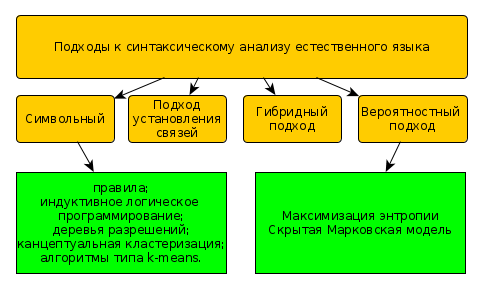
\includegraphics[width=\textwidth]{images/syntax_analysis_metods.png}
    \end{frame}
    \begin{frame}{Выбор средства синтаксического анализа}
        \begin{tabular}{|l|c|c|c|c|}
        \hline
                   & \cellcolor{blue!25} Stanford         & BLLIP             & Berkeley       &   Enju           \\
                   & \cellcolor{blue!25}Parser           & reranking         & Parser         &   parser         \\
                   & \cellcolor{blue!25}                 & parser            &                &                  \\ \hline

        тесты      & \cellcolor{blue!25}\small +         & \small +          & \small +       &\small -          \\ \hline

        значение   & \cellcolor{blue!25}\small +         & \small +          & \small +       &\small +          \\
        лексем     & \cellcolor{blue!25}                 &                   &                &                  \\ \hline

        лицензия   & \cellcolor{blue!25} \small GPLv2    & \small Apache v2  & \small GPLv2   & \small GPLv2     \\ \hline

        язык       & \cellcolor{blue!25}\small Java      & \small Python     &\small Java     &\small ---        \\ \hline

        связь      & \cellcolor{blue!25}\small отдель-   &\small вызов       &\small вызов    &\small отдель-    \\
        с          & \cellcolor{blue!25}\small ный       &\small на          &\small на       &\small ный        \\
        Moodle     & \cellcolor{blue!25}\small сервер    &\small сервере     &\small сервере  &\small сервер     \\ \hline

        зависимос- & \cellcolor{blue!25}\small +         & \small -          &\small -        &\small +          \\
        ти между   & \cellcolor{blue!25}                 &                   &                &                  \\
        лексемами  & \cellcolor{blue!25}                 &                   &                &                  \\ \hline
        подход к   & \cellcolor{blue!25}гибридный.       & вероят-           & символьный.    & установ-         \\
        синтакси-  & \cellcolor{blue!25}                 & ностный.          & k-best         & ление            \\
        ческому    & \cellcolor{blue!25}                 &                   & алгоритм       & связей.          \\
        анализу    & \cellcolor{blue!25}                 &                   &                & HPSG.            \\ \hline

        \end{tabular}
    \end{frame}
    \begin{frame}{Метод определения перечислений на основе синтаксического анализа}
        \begin{center}
            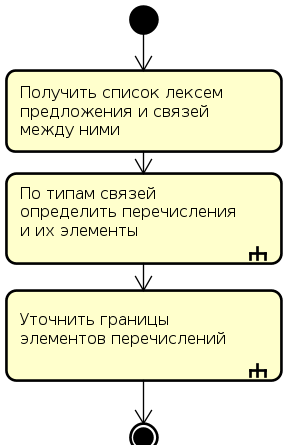
\includegraphics[height=0.7\textheight]{images/algorithm.png}
        \end{center}
    \end{frame}
    \begin{frame}{Метод определения перечислений на основе синтаксического анализа. Определение перечислений по типам связей лексем предложений.}
        \begin{center}
            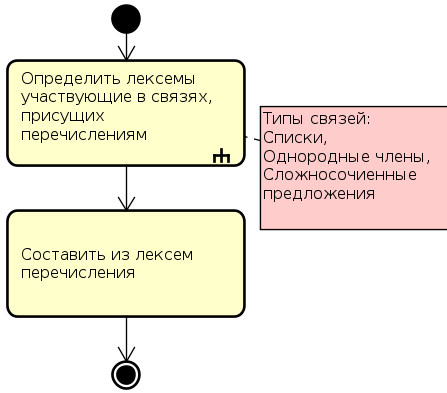
\includegraphics[height=0.7\textheight]{images/algorithm1.png}
        \end{center}
    \end{frame}
    \begin{frame}{Метод определения перечислений на основе синтаксического анализа. Уточнение границ элементов перечислений.}
        \begin{center}
            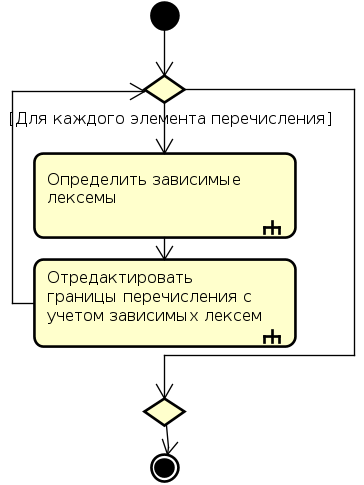
\includegraphics[height=0.7\textheight]{images/algorithm2.png}
        \end{center}
    \end{frame}
    \begin{frame}{План на летнюю практику}
        \Large
        \begin{enumerate}
            \item Написание 3 главы.
            \item Статья по результатам глав 1 и 2.
        \end{enumerate}
    \end{frame}
    \begin{frame}{Результаты семестра}
        \Large
        \begin{enumerate}
            \item Создано средство ввода тестов.
            \item Начат ввод тестов.
            \item Готовится статья по результатам 2-х семестров.
            \item Написана 1 глава.
        \end{enumerate}
    \end{frame}
    \begin{frame}{Научная новизна и практическая ценность}
        \begin{block} {Научная новизна работы} % (fold)
            \begin{enumerate}
                \item Использование метода определения перечислений на основе синтаксического анализа в новой области естественный языков.
                \item Разработанное метод позволяет с высокой точностью определить перечисления в предложении на естественном языке.
            \end{enumerate}
        \end{block}
        \begin{block}{Практическая ценность работы} % (fold)
            \par Реализованное программное средство позволяет проводить оценку ответа студента на естественном языке, с учетом содержания в ответе однородных членов и сложносочиненных предложений.
        \end{block}
    \end{frame}
    \begin{frame}{Список публикаций}
        \begin{enumerate}
            \item Готовится статья "Учет перечислений с произвольным порядком элементов при сравнении порядка лексем в тестовых вопросах с открытым ответом" в журнал "Вестник компьютерных и информационных технологий".
            \item Определение перечислений в предложениях на английском языке на основе их синтаксического анализа, Клевцов В.А., Внутривузовская научная конференция ВолгГТУ, Волгоград, 2016 г.
        \end{enumerate}
    \end{frame}
    \begin{frame}
        \begin{center}
            \Huge Спасибо за внимание!\\
            \LaTeX
        \end{center}
    \end{frame}
\end{document}
